\chapter{Conclusions}
\label{sec:concl}

For image processing, the more operations that can be parallelized, the faster images can be processed. However, as parallelism is increased, the amount of hardware required also is increased. It could be possible to parallelize a SAD algorithm, or most image processing methods, to only take a few clock cycles to process the whole image (i.e. every SAD calculation for an image pair happening simultaneously). Unfortunately, the area required on an FPGA would be a lot more than what was implemented in this paper. The cost of an FPGA that could handle that amount of hardware would be very cost prohibitive and not something a club or hobbyist could readily use for a robotics project. There does come a point at which the frames per second of disparity maps produced exceeds the speed that the other parts of the robot can process, which is unnecessary cost. So the FPGA board only needs to be able to handle a SAD implementation up to a certain frame rate, which depends on the requirements of the application for the robot.

The smaller the image size, the higher the frame rate, as shown in Figure~\ref{fig:frameRate}. Once the number of pixels in an image goes below 180,000 for the 7x7 window implementation or 140,000 for the 9x9 window implementation, the frame rate approaches 30 frames per second, which is good for humans. For robots, a frame rate of 10 should be sufficient for most tasks that do not require a higher frame rate. Both the 9x9 and 7x7 window implementations were shown be above 10 frames per second for an image size of 640x480.

\begin{figure}
	\begin{center}
		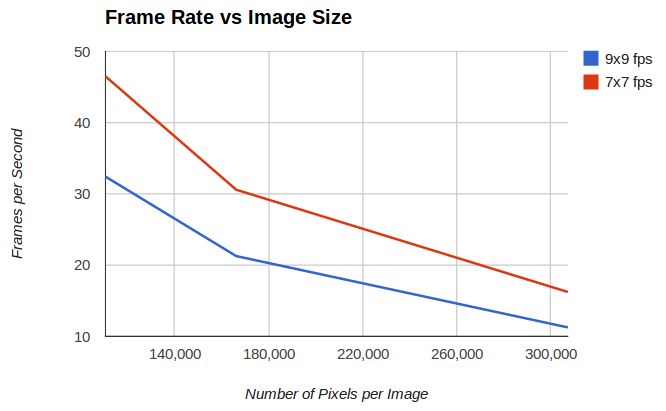
\includegraphics[width=100mm]{figures/frameRate.png}
		\captionfonts
		\caption{Frame rate comparison of different image sizes.}
		\label{fig:frameRate}
	\end{center}
\end{figure}

Between the 9x9 window implementation and the 7x7 window implementation, unless a higher frame rate is needed, the 9x9 is better than the 7x7. While 7x7 has a higher frame rate, 9x9 produces a better quality disparity map with less noise and requires fewer hardware resources.

This modular implementation of the SAD algorithm has the potential to be used for FPGA implementations in autonomous mobile robotic applications.